\documentclass[conference]{IEEEtran}

\usepackage{cite}
\usepackage{amsmath}
\usepackage{url}
\usepackage{hyperref}
\usepackage{booktabs}
\usepackage{multirow}
\usepackage{graphicx}
\usepackage{tikz}
\usetikzlibrary{arrows.meta,positioning,shapes.geometric}

\title{Reproducing Timeline Self-Reflection for Temporal Reasoning with LoRA Fine-Tuning}

\author{
\IEEEauthorblockN{
Gabriele Adorni s349308,
Berk Calisir s347896
Alessandro Casadei s349386, \\
Taha Atabay Cetin s349501,
Elias Noorzad s314515
}
\IEEEauthorblockA{
Politecnico di Torino\\
Deep Natural Language Processing\\
}
}

\begin{document}

\maketitle

\begin{abstract}
Temporal reasoning (tracking event order, duration, and overlap across a textual context) remains a difficult capability for large language models. This project reproduces the TISER framework proposed by Bazaga et al.~\cite{bazaga2025tiser}, which trains a model to generate an explicit structured trace (reasoning, timeline, reflection, answer) before producing its final response. We reproduce this setup using \texttt{Qwen2.5-7B-Instruct} with LoRA~\cite{hu2022lora} on the released TISER data (adapters on attention projections, $r{=}16$, $\alpha{=}32$, bf16, completion-only loss masking), reaching macro-EM~0.878 / macro-F1~0.949 on the full in-domain test set, in the same regime as the paper's 0.911~/~0.944 for the comparable configuration. Beyond reproduction, we propose a \emph{Context--Memory Conflict} probe: we select temporal-QA items the model reliably recalls closed-book (correct with no context at ${\geq}3/5$ self-consistency), then deterministically edit the context so the context-implied answer contradicts that memory. Across a $2{\times}2$ matrix of \{fine-tuned vs.\ vanilla\}${\times}$\{TISER vs.\ standard prompt\}, the TISER pipeline raises context-faithfulness from 0.380 to 0.787 (faithful-EM), but the \texttt{<reflection>} step almost never explicitly detects the contradiction: a Claude-based LLM-agent audit of all reflections puts the conflict-naming rate at 4.2\%, barely above the 2.3\% baseline revise-rate. TISER thus turns the model into a grounded reader, but not a genuine conflict auditor; order-reversal conflicts remain a blind spot where memorised answers dominate. A second extension adapts TISER to a tennis temporal-QA domain: the 7B TISER adapter transfers at EM~0.580, and continued tennis adaptation lifts it to EM~0.732 / F1~0.856.
The project repository is at \href{https://github.com/thestbobo/tiser_temporal_reasoning_extension}{GitHub repository}.
\end{abstract}

\section{Introduction}

Temporal reasoning, interpreting and manipulating time-related information such as event ordering, overlap, and duration, is central to temporal question answering, narrative understanding, and retrieval-augmented generation. Despite the strong general performance of recent large language models (LLMs), it remains fragile: models identify the relevant events but misalign them in time, confuse start and end points, or produce answers that are correct in content but not in the format expected by exact-match metrics.

TISER~\cite{bazaga2025tiser} improves temporal reasoning through explicit timeline self-reflection: instead of answering directly, the model is trained to produce a structured trace (an initial reasoning step, an explicit timeline of the relevant events, a reflection that checks the reasoning against the timeline, and a concise final answer) delimited by \texttt{<reasoning>}, \texttt{<timeline>}, \texttt{<reflection>}, and \texttt{<answer>} tags.

Our project reproduces the TISER baseline using \texttt{Qwen2.5-7B-Instruct} with LoRA fine-tuning on the released TISER data, then adds two extensions that are not part of the original paper. The first is a \emph{Context--Memory Conflict} probe: it asks whether the model follows the provided temporal context or its parametric memory when they disagree, and whether the \texttt{<reflection>} step explicitly detects the contradiction. This matters because TISER presents reflection as a mechanism for checking reasoning; our probe tests whether it also works as an auditing mechanism under adversarial conflict. The second is a tennis-domain adaptation study.

\section{Problem Statement}

\subsection{TISER Formulation}

We address temporal question answering over a textual or semi-structured temporal context. Each example consists of a question $q$, a temporal context $c$, and a gold answer $a$. The model is trained to generate a structured output $y = (r, t, s, a)$, where $r$ is the initial reasoning, $t$ is the explicit timeline, $s$ is the self-reflection, and $a$ is the final answer, serialized with the XML-like delimiters above. During evaluation, only the extracted \texttt{<answer>} span is scored.

The reproduction evaluates on five in-domain splits: TGQA~\cite{xiong2024tgqa}, TempReason L2 and L3~\cite{tan2023tempreason}, and TimeQA easy and hard~\cite{chen2021timeqa}. Out-of-distribution ToT-semantic examples are reported separately.

\subsection{Context--Memory Conflict Probe}

The extension probes whether the model follows a provided context or its memorised knowledge when they disagree. Given a real-entity temporal-QA item:
\begin{enumerate}
\item \textbf{Memory elicitation.} Remove the temporal context and elicit the model's closed-book answer $m$ via $k{=}5$ samples at temperature ${\approx}0.7$; accept the majority answer if it appears in ${\geq}3/5$ samples.
\item \textbf{Eligibility.} Keep only items where $m$ is confident and equals the original gold answer, ensuring a genuine memorised belief.
\item \textbf{Counterfactual construction.} Deterministically edit the context to produce $c'$ such that $\text{answer}(c') \neq m$.
\item \textbf{Evaluation.} Run the model on $(q, c')$ and score whether the prediction follows $c'$ or $m$.
\end{enumerate}

We define:
\emph{context-faithfulness} = prediction matches $\text{answer}(c')$;
\emph{memorisation} = prediction matches $m$;
\emph{conflict-detection} = \texttt{<reflection>} explicitly names the contradiction (decided by an LLM-agent audit, \S\ref{sec:methodology});
\emph{silent override} = faithful answer without explicit conflict detection.

We test three hypotheses. \textbf{H1:} the TISER prompt and fine-tune make the model more context-faithful under conflict than a plain prompt or the vanilla model. \textbf{H2:} when the model is faithful, the \texttt{<reflection>} step explicitly names the conflict (otherwise the faithfulness is a \emph{silent override}). \textbf{H3:} faithfulness depends on the \emph{type} of conflict (date-shift, entity-swap, or order-reversal). The full extension pipeline is summarised in Fig.~\ref{fig:pipeline}.

\subsection{Tennis Domain Adaptation}

The second extension asks whether TISER-style temporal reasoning transfers to professional-tennis narratives (before/after relations, first/last events, durations, tournament rounds): tennis-only LoRA adaptation at 0.5B scale and, at 7B scale, direct transfer of the original TISER adapter followed by continued tennis adaptation initialized from it.

\begin{figure}[t]
\centering
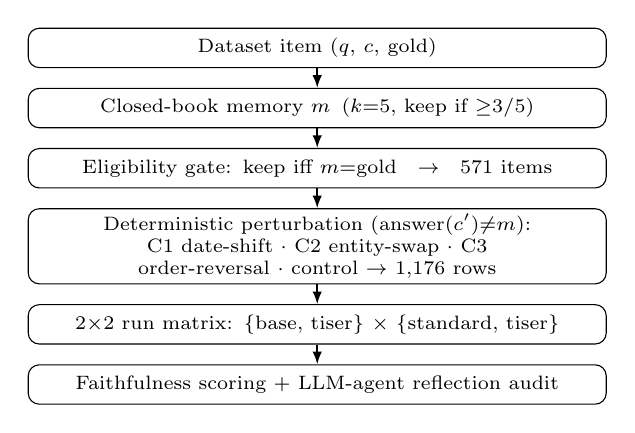
\begin{tikzpicture}[
  node distance=2.5mm,
  box/.style={draw, rounded corners, align=center, font=\scriptsize, text width=72mm, inner sep=2pt, minimum height=5mm},
  arr/.style={-{Latex[length=1.6mm]}, semithick}
]
\node[box] (n1) {Dataset item $(q,\,c,\,\text{gold})$};
\node[box, below=of n1] (n2) {Closed-book memory $m$\, ($k{=}5$, keep if ${\geq}3/5$)};
\node[box, below=of n2] (n3) {Eligibility gate: keep iff $m{=}\text{gold}\ \rightarrow\ 571$ items};
\node[box, below=of n3] (n4) {Deterministic perturbation ($\text{answer}(c'){\neq}m$): C1 date-shift $\cdot$ C2 entity-swap $\cdot$ C3 order-reversal $\cdot$ control $\rightarrow$ 1{,}176 rows};
\node[box, below=of n4] (n5) {$2{\times}2$ run matrix: \{base, tiser\} $\times$ \{standard, tiser\}};
\node[box, below=of n5] (n6) {Faithfulness scoring\ $+$\ LLM-agent reflection audit};
\draw[arr] (n1)--(n2);
\draw[arr] (n2)--(n3);
\draw[arr] (n3)--(n4);
\draw[arr] (n4)--(n5);
\draw[arr] (n5)--(n6);
\end{tikzpicture}
\caption{The inference-only Context--Memory Conflict pipeline: closed-book memory elicitation, an eligibility gate that keeps only confidently-recalled facts, deterministic counterfactual perturbation into conflict classes, a $2{\times}2$ model$\times$prompt run matrix, and faithfulness scoring plus an LLM-agent reflection audit.}
\label{fig:pipeline}
\end{figure}

\section{Methodology}
\label{sec:methodology}

\subsection{Baseline TISER Reproduction}

TISER decomposes temporal reasoning into four stages~\cite{bazaga2025tiser}: reasoning, timeline construction, reflection, and answer generation, all produced autoregressively in a single pass. The target supervision format teaches the model to externalize temporal structure before answering.

We use the Amazon-released TISER JSONL data. After a 2,048-token length filter, the training set contains 54,488 examples. The test set contains 22,014 examples (19,214 in-domain, 2,800 OOD ToT-semantic).

The base model is \texttt{Qwen2.5-7B-Instruct}, fine-tuned with LoRA~\cite{hu2022lora}: frozen base weights, trainable low-rank adapters on $q$/$k$/$v$/$o$ attention projections, rank $r{=}16$, scaling $\alpha{=}32$, dropout~0.05. Training uses bf16 precision without base quantization, 3 epochs, learning rate $2{\times}10^{-4}$, cosine schedule, warmup ratio~0.03, effective batch size~16, seed~42, and \texttt{paged\_adamw\_8bit}. Each training sample is converted into a Qwen chat-formatted prompt; the instruction/question/context tokens are masked with label $-100$ (completion-only loss). At inference, the model generates the full trace greedily (\texttt{max\_new\_tokens=768}), the \texttt{<answer>} span is extracted by regex, and the prediction is normalized using SQuAD-style normalization before computing Exact Match (EM) and token-level F1.

\paragraph{Setup.}
Fine-tuning ran on a single RunPod H200~SXM GPU (bf16 LoRA, no quantization; $54{,}488{\times}3$ epochs in ${\sim}6.5$\,h at ${\sim}7$ samples/s; seed~42) with PyTorch~2.4.1/CUDA~12.4, Transformers~4.46.3, PEFT~0.13.2, TRL~0.12.2. The full 22{,}014-example test evaluation and all probe inference ran on vLLM~0.22.0 (H100~SXM, bf16, greedy; PyTorch~2.11/CUDA~13.0): the full test pass takes ${\sim}17$\,min, the two closed-book memory-elicitation sweeps about 2\,h combined, and the four run-matrix cells minutes. The remaining stages (subset, eligibility, perturbation, scoring, the reflection-audit join and the analysis) are CPU-light and run locally.

\subsection{Extension: Context--Memory Conflict Probe}

The extension is inference-only (no new fine-tuning); the subject model is the frozen \texttt{Qwen2.5-7B-Instruct} + TISER adapter. Fig.~\ref{fig:pipeline} summarises the pipeline.

\paragraph{Subset, memory, eligibility (M0--M2).}
We keep the in-scope real-entity splits (TempReason L2/L3, TimeQA easy/hard; 15,898 items); TGQA is excluded as its synthetic/fictional entities lack the parametric belief needed for a knowledge-conflict probe. For each item the temporal context is deleted and the closed-book answer $m$ is elicited from $k{=}5$ samples at $T{\approx}0.7$, keeping the majority if it appears in ${\geq}3/5$ samples. An item is \emph{eligible} iff $m$ is confident and equals the original gold answer, ensuring a genuine memorised belief; this yields 571 eligible items.

\paragraph{Deterministic perturbation (M3).}
Each eligible item is edited into conflict classes:
\textbf{C1 (date-shift)} moves date ranges so a different entity covers the queried time-point;
\textbf{C2 (entity-swap)} replaces the answer entity with a same-type distractor;
\textbf{C3 (order-reversal)} swaps intervals so a before/after relation flips.
A \emph{control} arm reorders rows without changing the answer. Each edit enforces the invariant $\text{answer}(c'){\neq}m$, yielding 1,176 rows (C1 203, C2 520, C3 333, control 120) at 100\% per-class construction validity.

\paragraph{Run matrix (M4--M5).}
We cross \emph{model}~$\in$~\{vanilla Qwen (\texttt{base}), TISER fine-tuned (\texttt{tiser})\} with \emph{prompt}~$\in$~\{standard direct-answer, TISER 4-tag prompt\}; only TISER-prompt cells produce a \texttt{<reflection>} trace.

\paragraph{Scoring and reflection audit (M6--M7).}
M6 scores each prediction for faithful-EM/F1 (matches $\text{answer}(c')$), memorised-EM (matches $m$) and malformed rate. M7 is a separate post-hoc \emph{LLM-agent reflection audit}: a Claude-based agent reads each \texttt{<reflection>} from the TISER-prompt cells and returns a structured verdict (\texttt{conflict\_raised}, \texttt{conflict\_kind} $\in$ \{\texttt{timeline\_inconsistency}, \texttt{context\_error}, \texttt{context\_vs\_answer}\}, and a short rationale), processed in windows of 100 reflections. It judges the persisted traces only and supersedes a first-pass lexical mention proxy.

\subsection{Extension 2: Tennis Domain Adaptation}

The raw tennis set contains 1,122 temporal QA examples over professional-tennis narratives. Audit and conversion add ids, rule-based categories, prompts, and TISER-compatible fields; duplicate-aware splitting with seed~42 yields 785 train, 113 dev, and 224 test examples. The evaluator keeps the TISER trace format and parser and adds tennis-specific answer normalization (rankings, minute durations, punctuation, articles). At 0.5B we run base \texttt{Qwen2.5-0.5B-Instruct} with standard and TISER prompts, plus a tennis-only LoRA adapter trained on 600 trace-annotated examples. At 7B we transfer the original TISER adapter directly, then run continued tennis-from-TISER LoRA training initialized from it (a small grid over epochs, learning rate and batch size; each configuration trains in ${\sim}3$\,min). Mixed tennis+TISER replay and forgetting evaluation are out of scope.

\section{Experiments and Results}

\subsection{Baseline Reproduction}

Table~\ref{tab:baseline} reports our full in-domain test results. Our reproduction achieves macro-EM~0.878 / macro-F1~0.949 across the five in-domain splits. The original paper reports Qwen2.5-7B + TISER at macro-EM~0.911 / macro-F1~0.944 for the comparable in-domain configuration. Our result is in the same performance regime; remaining differences may stem from training infrastructure, data preprocessing, or stochastic variation.

\begin{table}[t]
\centering
\caption{Baseline reproduction on the full in-domain test set, against the paper's Qwen2.5-7B + TISER numbers. Macro is over the five in-domain splits; ToT-semantic (OOD, EM~0.381) is excluded.}
\label{tab:baseline}
\setlength{\tabcolsep}{4pt}
{\footnotesize
\begin{tabular}{lrcccc}
\toprule
\textbf{Split} & \textbf{$n$} & \textbf{EM} & \textbf{F1} & \textbf{Paper EM} & \textbf{Paper F1} \\
\midrule
TGQA            & 3{,}316 & 0.571 & 0.870 & 0.845 & 0.942 \\
TempReason L2   & 5{,}397 & 0.907 & 0.929 & 0.855 & 0.875 \\
TempReason L3   & 4{,}426 & 0.961 & 0.974 & 0.915 & 0.949 \\
TimeQA easy     & 2{,}997 & 0.980 & 0.989 & 0.979 & 0.983 \\
TimeQA hard     & 3{,}078 & 0.970 & 0.981 & 0.961 & 0.972 \\
\midrule
\textbf{Macro (5)} & 19{,}214 & \textbf{0.878} & \textbf{0.949} & 0.911 & 0.944 \\
\bottomrule
\end{tabular}
}
\end{table}

TGQA is the only split below the paper on EM (0.571) yet its F1 is high (0.870): in a 500-example audit of its predictions, ${\sim}56\%$ of the well-formed EM$=$0 cases are unit drops (e.g.\ ``8'' vs.\ ``8 years''). Crediting content-correct answers lifts effective TGQA accuracy to ${\approx}0.85$, matching the paper's 0.845, so the macro-EM gap is largely an exact-match formatting artifact rather than a reasoning gap.

\subsection{Context--Memory Conflict: Run Matrix}

Table~\ref{tab:conflict} reports faithfulness and memorisation rates across all four cells of the run matrix ($n{=}1{,}176$ conflict rows per cell).

\begin{table}[t]
\centering
\caption{Context--Memory Conflict run matrix. All metrics are rates over $n{=}1{,}176$ counterfactual items. The \emph{refl-conflict} column is the LLM-agent reflection audit, reported only for TISER-prompt cells.}
\label{tab:conflict}
\setlength{\tabcolsep}{3pt}
\begin{tabular}{llccccc}
\toprule
\textbf{Model} & \textbf{Prompt} & \textbf{faith-EM} & \textbf{faith-F1} & \textbf{mem-EM} & \textbf{malf.} & \textbf{refl-conf.} \\
\midrule
tiser  & tiser    & \textbf{0.787} & \textbf{0.917} & 0.230 & 0.002 & 0.042 \\
tiser  & standard & 0.574 & 0.771 & 0.297 & 0.000 & --   \\
base   & tiser    & 0.561 & 0.739 & 0.295 & 0.003 & 0.074 \\
base   & standard & 0.380 & 0.605 & 0.332 & 0.000 & --   \\
\bottomrule
\end{tabular}
\end{table}

The TISER prompt raises faithful-EM by $+0.213$ ($95\%$ CI $[+0.187,+0.238]$) on the fine-tuned model (0.787 vs.\ 0.574). Fine-tuning raises faithful-EM by $+0.225$ ($[+0.196,+0.254]$) under the TISER prompt (0.787 vs.\ 0.561). Both axes contribute substantially. Item-level bootstrap $95\%$ CIs (2{,}000 resamples, seed~42) on the four cells are $[.761,.810]$, $[.546,.603]$, $[.531,.589]$ and $[.352,.407]$, and both head-line gaps are significant under a paired McNemar test (prompt axis $\chi^2{=}219.9$; model axis $\chi^2{=}189.9$; both $p{<}10^{-40}$, $n{=}1{,}176$). The base model names conflicts in its reflection more often than the TISER fine-tune (7.4\% vs.\ 4.2\%, LLM-agent audit) yet is less faithful, so naming a conflict is not the same as resolving it. Fig.~\ref{fig:results} visualises both axes and the per-class breakdown.

\begin{figure}[t]
\centering
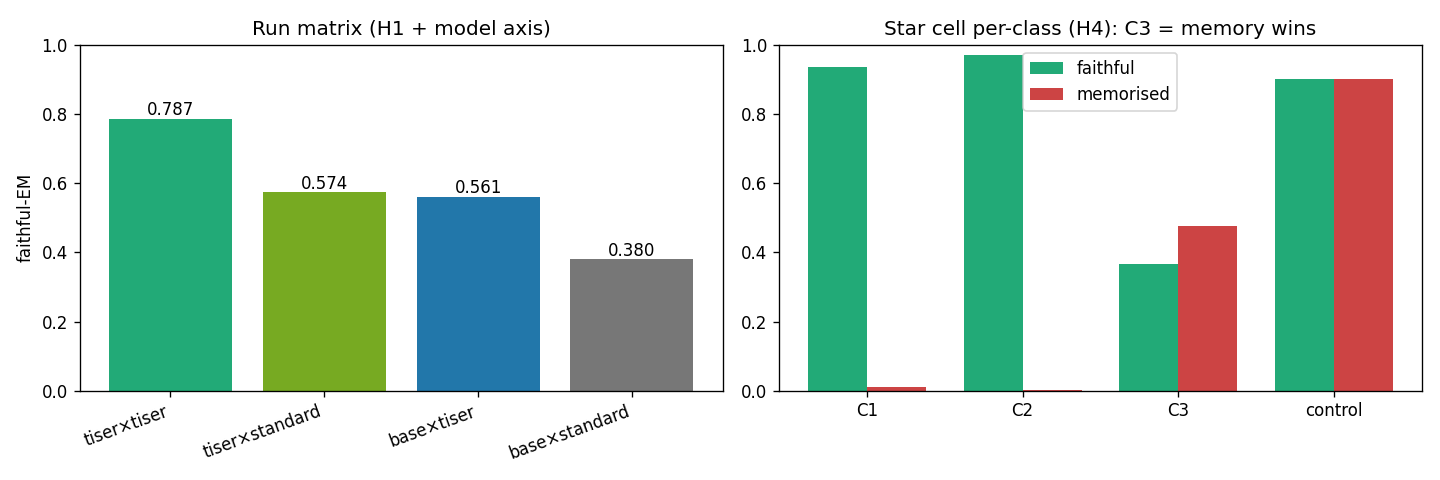
\includegraphics[width=\columnwidth]{figures/conflict_summary.png}
\caption{Left: faithful-EM across the $2{\times}2$ run matrix (the H1 prompt axis and the model/SFT axis). Right: per-class faithful vs.\ memorised EM for the star cell (tiser$\times$tiser); the C3 order-reversal bar is the only class where memory overtakes the text (H3).}
\label{fig:results}
\end{figure}

\subsection{Per-Conflict-Class Results (Star Cell)}

Table~\ref{tab:perclass} breaks down the star cell (\texttt{tiser}$\times$\texttt{tiser}) by conflict type.

\begin{table}[t]
\centering
\caption{Per-conflict-class results for the star cell (tiser$\times$tiser). \emph{agent-refl} is the LLM-agent conflict-naming rate. For \emph{control}, $\text{answer}(c'){\equiv}m$ by construction, so faithful- and memorised-EM coincide.}
\label{tab:perclass}
\setlength{\tabcolsep}{4pt}
{\footnotesize
\begin{tabular}{lrcccl}
\toprule
\textbf{Class} & \textbf{$n$} & \textbf{faith-EM} & \textbf{mem-EM} & \textbf{agent-refl} & \textbf{Reading} \\
\midrule
C1 date-shift      & 203 & 0.936 & 0.010 & 0.020 & follows text \\
C2 entity-swap     & 520 & 0.971 & 0.002 & 0.008 & follows text \\
C3 order-reversal  & 333 & 0.366 & 0.477 & 0.111 & memory wins  \\
control            & 120 & 0.900 & 0.900 & 0.033 & sanity floor \\
\bottomrule
\end{tabular}
}
\end{table}

C1 (date-shift) and C2 (entity-swap) are largely solved: the fine-tuned model reliably follows the edited text (faithful-EM~${\geq}0.936$). C3 (order-reversal) is the blind spot, where faithfulness collapses to 0.366 and memorised answers overtake faithful ones (0.477 vs.\ 0.366). The audit ties H2 to H3: the model raises the clash almost only on C3 (11.1\%, vs.\ ${\leq}2\%$ on C1/C2), so it tends to notice exactly the class it fails. The control arm is a sanity floor: $\text{answer}(c'){\equiv}m$ by construction, so faithful- and memorised-EM coincide (0.900), measuring only whether a benign edit preserved answerability. Control is also an L3-heavy subsample (58\% TempReason-L3) and not prompt-independent (0.700 under the standard prompt), so it does not prove the edits universally clean.

\subsection{Tennis Domain Adaptation}

Table~\ref{tab:tennis} reports the completed 224-example tennis-test runs at both scales; smaller smoke conditions are not treated as final results.

\begin{table}[t]
\centering
\caption{Tennis temporal QA on the 224-example test set. Deltas are against each block's first row (0.5B: base with standard prompt; 7B: direct transfer of the original TISER adapter).}
\label{tab:tennis}
\setlength{\tabcolsep}{3pt}
{\footnotesize
\begin{tabular}{lccccc}
\toprule
\textbf{Condition} & \textbf{EM} & \textbf{F1} & \textbf{$\Delta$EM} & \textbf{$\Delta$F1} & \textbf{Malf.} \\
\midrule
\multicolumn{6}{l}{\emph{Qwen2.5-0.5B-Instruct}} \\
Base, standard prompt   & 0.379 & 0.472 & -- & -- & 0 \\
Base + TISER prompt     & 0.375 & 0.420 & $-$0.004 & $-$0.052 & 5 \\
Tennis-only adapter     & 0.464 & 0.516 & $+$0.085 & $+$0.045 & 0 \\
\midrule
\multicolumn{6}{l}{\emph{Qwen2.5-7B-Instruct}} \\
Original TISER transfer & 0.580 & 0.701 & -- & -- & 0 \\
Best tennis-from-TISER  & \textbf{0.732} & \textbf{0.856} & $+$0.152 & $+$0.155 & 0 \\
\bottomrule
\end{tabular}
}
\end{table}

\section{Analysis}

\subsection{Context--Memory Conflict}

\textbf{H1 (context-faithfulness) is supported.} The TISER prompt and TISER fine-tuning independently increase context-faithfulness under conflict, jointly raising faithful-EM from the base-standard floor of 0.380 to 0.787.

\textbf{H2 reveals silent override.} The TISER fine-tuned model often follows the edited context (78.7\%) but almost never explicitly notices that the context contradicts its memorised belief: an LLM-agent audit of all 1,176 reflections puts the conflict-naming rate at 4.2\%, barely above the 2.3\% baseline revise-rate measured on normal (non-conflict) data. This rare noticing is driven by conflict \emph{type}, not memory strength: it concentrates on C3, is non-monotonic in the closed-book self-consistency score (peaking at 4/5, not 5/5), and even when a clash is flagged the answer reverts to memory in 23 of the 49 flagged star-cell rows. TISER turns Qwen into a grounded reader, but not a genuine auditor.

\textbf{H3 (conflict-type dependence) is supported.} Date-shift and entity-swap conflicts are nearly solved (faithful-EM $\geq$~0.936), while order-reversal collapses faithfulness: it is the only class where memorised-EM exceeds faithful-EM.

\subsection{Tennis}

At 0.5B, TISER prompting alone does not help (F1 drops, five malformed outputs): the trace format costs a small model more than it buys, while tennis-only adaptation gives a modest +0.085 EM. The useful result is at 7B: the TISER adapter transfers at EM~0.580 and continued adaptation reaches 0.732, a genuine domain-adaptation gain on top of transfer. Forgetting on the original TISER data was not evaluated, so preservation of general performance remains open.

\subsection{Caveats}

Conflict-naming is decided by a single automated LLM-agent judge; it agrees with the discarded keyword proxy only moderately (Cohen's $\kappa{=}0.76$ on the star cell), with no second judge or human calibration. The eligible set is biased toward facts the model already knows confidently, so 0.787 faithful-EM characterises performance on strong memory conflicts, not a random sample of all temporal QA. All cell scores are single greedy decodes, though we report item-level bootstrap CIs and paired McNemar tests for the headline comparisons. Finally, reflection text is not mechanistically faithful reasoning.

\section{Conclusions}

Our reproduction of TISER under a single-GPU LoRA setup succeeds, reaching macro-EM~0.878 / macro-F1~0.949 on the full in-domain test set.

The Context--Memory Conflict extension shows that TISER substantially improves context-faithfulness under counterfactual contexts: faithful-EM rises from 0.380 (vanilla baseline) to 0.787 (TISER fine-tune + TISER prompt). However, the reflection stage mostly rubber-stamps the answer rather than naming the contradiction (4.2\% vs.\ a 2.3\% baseline revise-rate), and event-ordering conflicts remain a weakness where the model reverts to memorised temporal order. The tennis extension shows that the 7B TISER adapter transfers to an unseen sports domain (EM~0.580) and that continued adaptation adds a further +0.152 EM, while at 0.5B the TISER prompt alone is not beneficial.

The main practical challenges were exact-match brittleness, full-test generation throughput (solved with vLLM), and building perturbations whose validity is checkable by construction. The main lesson is that behavioural grounding and introspective transparency are separate capabilities: improving one does not imply the other.

\section{Reproducibility}

The pipeline is config-driven (\texttt{config/config.yaml}, \texttt{config/conflict.yaml}, tennis configs) with fixed seed~42; every run saves \texttt{run\_meta.json} (git SHA, library versions, resolved config), predictions, and per-example scores. Each conflict stage (M0--M7, M10 stats) writes its artifact and meta under \texttt{outputs/conflict/<stage>/}, and headline metrics are mirrored under \texttt{results/}. Source code and this report are in the \href{https://github.com/thestbobo/tiser_temporal_reasoning_extension}{project repository}.

\begin{thebibliography}{00}

\bibitem{bazaga2025tiser}
A. Bazaga, R. Blloshmi, B. Byrne, and A. de Gispert,
``Learning to Reason Over Time: Timeline Self-Reflection for Improved Temporal Reasoning in Language Models,''
in \emph{Proceedings of ACL}, 2025.

\bibitem{xiong2024tgqa}
S. Xiong, A. Payani, R. Kompella, and F. Fekri,
``Large Language Models Can Learn Temporal Reasoning,''
in \emph{Proceedings of ACL}, 2024.

\bibitem{tan2023tempreason}
Q. Tan, H. T. Ng, and L. Bing,
``Towards Benchmarking and Improving the Temporal Reasoning Capability of Large Language Models,''
in \emph{Proceedings of ACL}, 2023.

\bibitem{chen2021timeqa}
W. Chen, X. Wang, and W. Y. Wang,
``A Dataset for Answering Time-Sensitive Questions,''
in \emph{NeurIPS Datasets and Benchmarks}, 2021.

\bibitem{hu2022lora}
E. J. Hu et al.,
``LoRA: Low-Rank Adaptation of Large Language Models,''
in \emph{International Conference on Learning Representations}, 2022.

\end{thebibliography}

\end{document}